%
% Revision 30 Nov 2023
%
%%%%%%%%%%%%%%%%%%%%%%%%%%%%%%%%%%%%%%%%%%%%%%%%%%%%%%%%%%%%%%%%%%%%%%%%%%%%%%%%
%2345678901234567890123456789012345678901234567890123456789012345678901234567890
%        1         2         3         4         5         6         7         8
% DOCUMENT CLASS
\documentclass[a4paper,12pt]{Classes/RoboticsLaTeX}

% USEFUL PACKAGES
% Commonly-used packages are included by default.
% Refer to section "Book - Useful packages" in the class file "Classes/RoboticsLaTeX.cls" for the complete list.
\usepackage{amsmath}
\usepackage{amsfonts}
\usepackage{algorithm}
\usepackage{algorithmic}
\usepackage{multirow}
\usepackage{colortbl}
\usepackage{color}
\usepackage[table]{xcolor}
\usepackage{epigraph}
\usepackage{graphicx}
%\usepackage{subfigure}
\usepackage{caption}
\usepackage{subcaption}
\usepackage{hyperref}
\usepackage{tabularx}
\usepackage{float}
\usepackage{longtable}
\usepackage[pdftex]{graphicx}
\usepackage{pdfpages}
\usepackage{pdflscape}
\usepackage[acronym,toc]{glossaries}
\usepackage{setspace}
\usepackage[utf8]{inputenc}
\usepackage[table]{xcolor}

%\usepackage{layout}

\setstretch{1.5}
%\onehalfspacing

% SPECIAL COMMANDS
% correct bad hyphenation
\hyphenation{op-tical net-works semi-conduc-tor}
\hyphenation{par-ti-cu-lar mo-du-le ge-stu-re}
% INTERLINEA 1.5
%\renewcommand{\baselinestretch}{1.5}

%% ignore slightly overfull and underfull boxes
%\hbadness=10000
%\hfuzz=50pt
% declare commonly used operators
%\DeclareMathOperator*{\argmax}{argmax}

% >>>> Replace all the [[Placeholders]] on the front page and in the Declaration <<<<

\title{\Large{[[Thesis Title]]}}

\author{[[NAME]]}
\collegeordept{School of Computer Science}
\university{University of Galway}
\crest{
\includegraphics[width=135mm]{Figures/University_Of_Galway_Logo__Positive_Landscape.png}}
%\crest{
\includegraphics[width=80mm]{Figures/University_of_Galway_logo_2022.png}}

\supervisor{[[Name(s) of Supervisor(s)]]}
%\supervisor{Name of the Supervisor}
%\supervisor{Name of the Co-Supervisor}	

% replace NAME with your name and PROGRAMME with Data Analytics, Artificial Intelligence, or Artificial Intelligence - Online
\degree{MSc in Computer Science ([[PROGRAMME]])}
\degreedate{[[Date of submission]]}  % Replace with submission date


%%%%%%%%%%%%%%%%%%%%%%%%%%%%%%%%%%%%%%%%%%%%%%%%%%%%%%%%%%%%%%%%%%%%%%%%%%%%%%%%
%%% uncomment if glossary needed, see examples in file
%\makeglossaries
%\loadglsentries{glossary}

\begin{document}
	\begin{spacing}{1}
		\maketitle
	\end{spacing}
	
	% add an empty page after title page
	\newpage\null\thispagestyle{empty}\newpage
	
	% set the number of sectioning levels that get number and appear in the contents
	\setcounter{secnumdepth}{3}
	\setcounter{tocdepth}{3}
	
	\frontmatter
	
	% Replace NAME and THESIS-TITLE with your name and the title of this thesis.
	\textbf{DECLARATION} 
	I, [[NAME]], hereby declare that this thesis, titled ``[[THESIS-TITLE]]'', and the work presented in it are entirely my own except where explicitly stated otherwise in the text, and that this work has not been previously submitted, in part or whole, to any university or institution for any degree, diploma, or other qualification. 
	\newline
	
	\begin{tabular}{@{}p{.5in}p{4in}@{}}
		Signature: & ~~\hrulefill \\
	\end{tabular}
	\newpage
	
	
	%%%% uncomment if acknowledgements needed
	%\textbf{Acknowledgement}
	%
	%
	%\newpage\textbf{}
	
	
	% THESIS ABSTRACT
	\begin{abstracts}
		The abstract should summarise the substantive results of the work and not merely list topics to be discussed. An abstract is an outline/brief summary of your thesis and your whole project. 
		
		It should be terse and usually written in the present tense: ``A new graph community detection algorithm is proposed based on spectral features. It is compared against several strong baselines ...''.
		
		As everywhere in the thesis, sources need to be cited (using \texttt{\textbackslash cite}).
		
		\textbf{Keywords: } Keyword1, Keyword2, Keyword3, Keyword4, Keyword5
	\end{abstracts}
	
	
	\tableofcontents
	\listoffigures
	\listoftables
	\printglossary[title=List of Acronyms,type=\acronymtype]
		
	
	\mainmatter
	
	
	\chapter{Introduction}
	\label{chap:introduction}
	
	This chapter should be short and highly readable, even to non-experts. It should describe the topic of the project and the research problem it tackles, motivate your research, and include precise \textit{research questions} or \textit{hypotheses} you aim to answer or test, respectively, with your research).\\
	
	\noindent A typical structuring of the Introduction chapter:
	\begin{itemize}
		\item Topic and purpose of your project. What problem(s) does your project tackle? 
		\item \textit{Motivation}. Why is your project important? What is the research area (within AI/DA) to which your project belongs (describe the area)? How does your project relate to existing research in that area? What ``gap'' in existing research does your project address\footnote{Identifying this ``gap'' is an important outcome of your Literature Review, see Chapter 3.}?
		\item The \textit{Research Questions} your project aims to answer, and how. Research questions are typically numbered \textbf{RQ1}, \textbf{RQ2}, \textbf{RQ3}, ...
		\item Structure of the thesis (what each of the following chapters is about. E.g., {\em The next chapter provides an overview of ... Chapter 3 discusses ...})
	\end{itemize}
	
	
	------------------------------------------------------------------------------------
	
	\underline{Remark}: The chapters and sections recommended in this thesis template are very common, but it is not the only valid thesis structure. You should discuss the thesis structure with your supervisor when you draft your Project Proposal (PP) document. \textbf{Also take a look at sample MSc AI and MSc Data Analytics theses from previous years (available on Canvas) for typical ways of structuring a thesis.}\\
	
	The following is a guideline for number of pages per chapter:
	
	\begin{itemize}
		\item Abstract 1 
		\item Introduction 3-4
		\item Background 3-5
		\item Related work 3-6
		\item Data 1-3
		\item Methodology 6-10
		\item Experiments 2-3
		\item Results 4-10
		\item Conclusion 1-2
	\end{itemize}
	
	(in total 24-44 pages, without title page, declaration page, Table of Contents, List of Figures, List of Tables, Bibliography)
	
	\textbf{Observe the normally expected minimum number of words as well as the strict upper limit for the number of words in your thesis (see thesis guidelines document).}\\
	
	We have given Chapter titles, but you should also use \verb+\section+ and \verb+\subsection+ to give chapters a more fine-grained structure as needed.
	
	You can refer to other chapters/sections using \verb+\ref+, e.g.~``We will describe the proposed new model in detail in Chapter~\ref{chap:methodology}.''\\
	
	Notice that we must use paired backquotes and apostrophes for correct quotation marks in Latex: ``here is an example''. If we use standard quotation marks they are formatted incorrectly: "here is an example".
	
	Simple equations are written using \verb+$...$+, e.g.~$e^{i\pi} - 1 = 0$.\\
	
	Figures should be formatted using \verb+\begin{figure}...\end{figure}+, with captions and labels. Figures should then be referred to from the text, e.g.: Figure~\ref{fig:penrose} shows an example of a logo.
	\begin{figure}
		\centering
		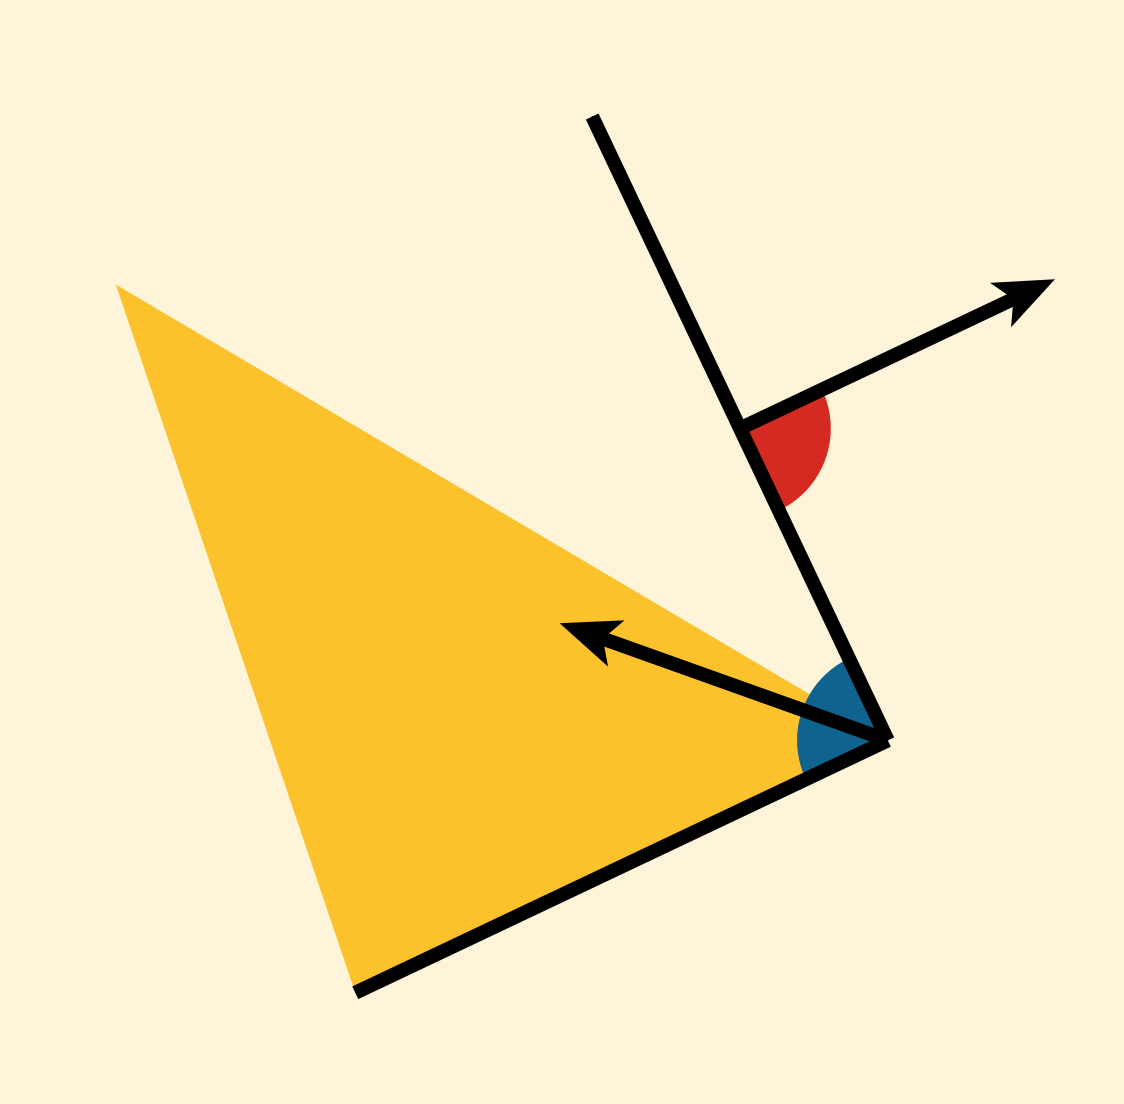
\includegraphics[width=0.3\linewidth]{Figures/penrose.png}
		\caption{A suitable caption. Image from \cite{10.1145/3386569.3392375}. Keep in mind that all images, graphs, tables and other figures not created by yourself require that you state their {[sources]} (using \texttt{\textbackslash cite}).}
		\label{fig:penrose}
	\end{figure}
	
	\vspace{2ex} Refer to Overleaf documentation (\verb#https://www.overleaf.com/learn/latex#) and other online resources for basic LaTeX usage, in particular mathematics, emphasis, and citation.\\

	\textbf{Remember that in the thesis as well as in the Project Proposal, \underline{all} existing  text, ideas, concepts, facts, results, images, graphs, data, program code, algorithms, approaches, methods and other content, must be properly cited with the exact sources. }\\
	
	If you paste any text from any source, you must quote (put the original text in ``quotation marks'') and cite (\texttt{\textbackslash cite}). 
	
	Do \underline{not} paste any text and then alter it to avoid quoting and citing. Instead, you need to restate the meaning of the text \underline{entirely in your own words} (\textit{paraphrasing}) and cite the source. Alternatively, use a ``direct quote'' and cite the source (but normally paraphrasing is preferred, unless the preservation of the exact words of the original text is essential). Both paraphrasing and quoting require that the source is cited (using \texttt{\textbackslash cite}).\\
	
	
		\textbf{Carefully familiarize yourself with the referencing style (citation style) you are planning to use.} Unless a different referencing style is stipulated by your supervisor, it is strongly recommended to use \textbf{IEEE style} (the most common referencing style in Computer Science):\\ \verb#https://libguides.ncirl.ie/referencingandavoidingplagiarism/ieee#\\
	
	\noindent Also familiarise yourself with BibTeX (see below).\\
	
	For citations, use \verb#\cite# commands. Example:\\
	\verb#Community detection in graphs is an interesting problem \cite{NewmanGirvan2004}.#
	will appear as\\
	Community detection in graphs is an interesting problem \cite{NewmanGirvan2004}.
	
	To include page numbers (for direct quotes, or when referencing content in books or long articles), use, e.g.,\\ \noindent \verb#\cite[p.~22]{NewmanGirvan2004}# (appears as \cite[p.~22]{NewmanGirvan2004}).
	
	To combine multiple references, separate the citation-keys by commas, e.g.,\\ 
	\noindent \verb#\cite{NewmanGirvan2004,DBLP:books/aw/RN2020}#, which will appear as \cite{NewmanGirvan2004,DBLP:books/aw/RN2020}.\\
	
 Do not write paper titles, e.g.~do not write {\em In a paper titled ``Community Detection in Graphs'' \cite{NewmanGirvan2004}, the authors propose a new approach to ...}. Just cite (e.g., {\em In \cite{NewmanGirvan2004}, the authors propose a new approach to ...}).\\
	
	%There are two styles, depending on your sentence:
	%\begin{itemize}
	%\item Parenthetical \verb+\citep{NewmanGirvan2004}+: Community detection in graphs is an interesting problem \citep{NewmanGirvan2004}.
	%\item Textual \verb+\citet{NewmanGirvan2004}+: It was shown by \citet{NewmanGirvan2004} that community detection in graphs is an interesting problem.
	%\end{itemize}
	
	\textbf{It is strongly recommended to use BibTeX for references.} Add your sources (bibliography items), such as papers, articles, books, web pages... to file references.bib. BibTeX items for articles, books and papers can often be found on the Web (but you still need to check their correctness and completeness, and amend/complete if necessary). A good tutorial about BibTeX is\\
	\verb#https://www.overleaf.com/learn/latex/Bibliography_management_with_bibtex#
	
	\chapter{Background}
	\label{chap:backg}
	
	Here you can give textbook-level knowledge which you might expect that expert researchers can skip but might be helpful to establish the setting and terminology. 
	
	You can also give some general knowledge, e.g., the number of people affected by some issue, the number of users of some website, or the size of some industry, to help motivate the importance (but remember that you should motivate your project also, in short form, in the Introduction).\\
	
	Sometimes this chapter is combined with the ``Related Work'' chapter to a single chapter named, e.g., ``Background and Related Work'' or ``Literature Review''.
	
	\chapter{Related Work}
	\label{chap:rel_work}
	
	The Related Work chapter provides a survey of scholarly articles, conference papers, books and other existing works relevant to the topic of your thesis. It provides context for your own research, allows to identify the state-of-the-art (current knowledge about the matter of the thesis) and a ``gap'' in existing research your thesis aims to close.\\
	
	It should stick to relevant and scholarly papers and articles. \\
	
	Learn to recognise and avoid spam/predatory/pay-to-publish/vanity journals and conferences. Use newspaper/magazine/blog/tutorial sources only very rarely and only if truly unavoidable. Cite the originator of an idea, not a random author who used it recently.\\
			
	The Related Work chapter should be synthetic, that is it should identify common themes and issues and connections between papers to form a larger-scale understanding. It should help the reader by giving a taxonomy or categorisation of existing work, i.e.~it should not be a bare list of papers. \textbf{It should demonstrate critical thinking and judgement, not just rephrase what previous authors have claimed.} \\
			
	\chapter{Data}
	\label{chap:data}
	
	You might need a chapter (or, alternatively, a section in chapter ``Methodology'') about your data, its characteristics and pre-processing. This chapter is particularly relevant if you are using a dataset that has not been previously described in detail.\\
	
	But even if you do not use a dedicated ``Data'' chapter, you still need to describe all datasets you are using (e.g., in chapter ``Methodology'').\\
	
	\noindent Existing datasets need to be cited with the exact sources.
	
	\chapter{Methodology}
	\label{chap:methodology} 
	
	Here you describe your approach to your research, and your reasoning behind your approach.\\
	
	For example, what kind of data you use, and why is this data appropriate? How is the data collected, sampled or generated, and why is this approach appropriate?\footnote{Alternatively, the data can be described in a dedicated chapter ``Data''} \\
	
	What methods do you use to process and analyse your data, and why are those methods appropriate? What are the limitations of your methods and data? \\
	
	What models, algorithms, processes, code, software frameworks or tools did you use or create? Describe them, and justify your choices and designs. \\
	
	In this and the remaining chapters, \underline{relate}, where appropriate, the approaches you used, the decisions you made and the results you obtained \underline{to your Research Questions} from the Introduction. E.g., ``To answer RQ1, we firstly train a Convolutional Neural Network using a large set of cat images...''.\\
	
		Program source code should normally not be put in the thesis body, or only sparingly (noteworthy code snippets). Provide the link to a source repository (e.g., on GitHub) for the complete source code. Also, relevant source code can be put in an appendix\footnote{Appendices (numbered Appendix A, Appendix B, ...) provide supplementary information to the thesis and appear after the Bibliography (References).} to which you refer from the main body of the thesis (but the full source code still needs to be made available to the supervisor and second marker as files on, e.g., GitHub, as described in the Project Guidelines).
	
	\chapter{Experiments}
	\label{chap:experiments}
	
	Give a complete technical description of your experiments, sufficient for another researcher to understand your experimental approach and reproduce your results. \\
		
	\noindent \textbf{(Note that experimental \textit{results} and their discussion belong in the next chapter.)} 
	
	\chapter{Results}
	\label{chap:results}
	
	Results first, using figures and tables, with little commentary and no interpretation.
	
	\noindent Then detailed analysis and interpretation.\\
	
	\textbf{Link experimental results to your \underline{research questions}} or hypotheses, e.g., ``The results in Table 3 clearly show that the answer to RQ2 is negative ...''.
	
	\chapter{Conclusion}
	\label{chap:conclusion}
	
	Here you must zoom back out to evaluate the thesis itself. Mention its contributions and main results (in brief form), its limitations and weaknesses, and possible future work.
	
	%%%%%%%%%%%%%%%%%%%%%%%%%%%%%%%%%%%%%%%%%%%%%%%%%%%%%%%%%%%%%%%%%%%%%%%%%%%%%%%%
	%\bibliographystyle{plainnat}                  % to give author-year style
	\bibliographystyle{IEEEtranN} 
	\renewcommand{\bibname}{References}           % change default name Bibliography to References
	\bibliography{references}                     % BibTeX References file, references.bib
	\addcontentsline{toc}{chapter}{References}    % add References to TOC
	
	
	%%% uncomment if Appendices needed
	%\appendix
	%\chapter{Appendix-A-Title} 
	%\label{chap:appendix_a}
	
	%\chapter{Appendix-B-Title} 
	%\label{chap:appendix_b}
	
\end{document}
